\documentclass[11pt,a4paper]{article}
\usepackage[utf8]{inputenc}
\usepackage[T1]{fontenc}
\usepackage[french]{babel}
\usepackage{lmodern}
\usepackage{geometry}
\geometry{margin=2.1cm}
\usepackage{microtype}
\usepackage{setspace}
\setstretch{1.08}
\usepackage{xcolor}
\definecolor{cpblue}{HTML}{244A73}
\definecolor{cpgreen}{HTML}{2E7D6E}
\definecolor{cporange}{HTML}{C06B28}
\definecolor{cpgray}{HTML}{F3F5F7}
\definecolor{cpdark}{HTML}{24313B}
\usepackage{tikz}
\usetikzlibrary{arrows.meta,positioning,shapes.geometric,fit,calc}
\usepackage{booktabs}
\usepackage{tabularx}
\usepackage{array}
\usepackage{longtable}
\usepackage{amsmath,amssymb}
\usepackage{enumitem}
\usepackage{hyperref}
\hypersetup{colorlinks=true,linkcolor=cpblue,urlcolor=cpblue,citecolor=cpblue}
\usepackage{fancyhdr}
\usepackage{subcaption}
\pagestyle{fancy}
\fancyhf{}
\lhead{Documentation SCONTO-SVU}
\rhead{Module de prévision Prophet / Recalibrator / DataCo}
\cfoot{\thepage}
\setlength{\headheight}{14pt}
\usepackage{titlesec}
\titleformat{\section}{\Large\bfseries\color{cpblue}}{\thesection}{0.6em}{}
\titleformat{\subsection}{\large\bfseries\color{cpdark}}{\thesubsection}{0.6em}{}
\usepackage{caption}
\usepackage{graphicx}
\usepackage{float}
\captionsetup{font=small,labelfont=bf}
\newcommand{\code}[1]{\texttt{#1}}
\newcommand{\pill}[1]{\tikz[baseline=(X.base)]\node[rounded corners=2pt,fill=cpgray,inner xsep=4pt,inner ysep=1.5pt] (X) {\footnotesize\texttt{#1}};}

\begin{document}

\begin{titlepage}
\centering
\vspace*{2.2cm}
{\Huge\bfseries\color{cpblue} Module de prévision et d'exécution DataCo\par}
\vspace{0.45cm}
{\LARGE Prophet, Recalibrator et génération automatique de la demande\par}
\vspace{1.3cm}
{\large Documentation technique du modèle SCONTO-SVU\par}
\vspace{1.6cm}
\begin{tikzpicture}[node distance=10mm,>=Latex]
\tikzset{
 box/.style={draw=cpblue,rounded corners,minimum width=3.5cm,minimum height=1.05cm,align=center,fill=cpgray},
 arrow/.style={->,thick,draw=cpdark}
}
\node[box] (prophet) {Prévision Prophet\\2017};
\node[box,right=of prophet] (real) {Demande réelle\\\code{CommandeAgent}};
\coordinate (titlemid) at ($(prophet)!0.5!(real)$);
\node[box,below=10mm of titlemid] (recal) {Recalibrator\\prévision ajustée};
\draw[arrow] (prophet) -- (recal);
\draw[arrow] (real) -- (recal);
\node[box,below=of recal] (kpi) {Écarts dynamiques\\et visualisation};
\draw[arrow] (recal) -- (kpi);
\draw[arrow] (real) |- (kpi);
\end{tikzpicture}
\vfill
{\large Prévision, exécution multi-produit et recalibration adaptative de la demande\par}
\vspace{0.5cm}
{\small Le module s'appuie sur le pipeline VSM/SCOR de SCONTO-SVU : DataCo alimente la demande à travers le traitement normal des commandes.\par}
\end{titlepage}

\tableofcontents
\newpage

\section{Objectif du module}

Le module de prévision complète le modèle SCONTO-SVU par une chaîne intégrée qui prévoit la demande, rejoue une demande réaliste issue de DataCo, observe la demande réellement générée dans la simulation, puis réajuste progressivement la prévision au cours du mois.

L'intégration poursuit quatre objectifs principaux :
\begin{itemize}[leftmargin=1.5em]
  \item conserver une \textbf{prévision Prophet de référence} calculée sur les données historiques DataCo ;
  \item fournir un mode \textbf{DataCo} qui génère automatiquement les commandes clientes à partir d'une calibration historique ;
  \item calculer une \textbf{prévision recalibrée} à mesure que la demande réelle devient observable ;
  \item visualiser dynamiquement \textbf{Prophet, Recalibrator, demande réelle et écarts} pendant l'exécution.
\end{itemize}

DataCo n'est pas une troisième prévision : il constitue la source qui génère les commandes formant le \emph{réel simulé}. Les deux prévisions comparées tout au long de ce document restent donc \textbf{Prophet} et \textbf{Recalibrator}.

\medskip
\noindent\fcolorbox{cpblue}{cpgray}{\begin{minipage}{0.965\textwidth}
\small
\textbf{Portée du module.} Prophet, le Recalibrator et l'AutoCommande DataCo forment une instanciation expérimentale du modèle SCONTO-SVU pour le cas DataCo : le noyau générique du modèle (\code{model/SCONTO\_SVU\_GENERIC\_MASTER.alp}) reste piloté par des scénarios JSON génériques, et cette instanciation le complète par un module de prévision et de recalibration de la demande. La version décrite ici correspond fonctionnellement à la déclinaison \code{SCONTO\_SVU\_FINAL\_\allowbreak VALIDATED\_FORECAST\_\allowbreak DATACO\_MULTIPRODUCT\_\allowbreak CONCURRENT\_FIX.alp}.
\end{minipage}}
\medskip

\noindent\textit{Identification du modèle exécuté.} Le manifeste runtime des campagnes RUN 1 et RUN 2 déclare un champ \code{modeleCandidate = SCONTO\_SVU\_FINAL\_\allowbreak VSM\_FIX\_\allowbreak CANDIDATE.alp}. La comparaison de contenu montre qu'il s'agit d'une étiquette de traçabilité codée en dur dans le générateur de manifeste, présente à l'identique dans plusieurs variantes du dépôt, et non du nom de fichier réellement chargé lors de l'exécution : le fichier \code{sources/model/\allowbreak SCONTO\_SVU\_FINAL\_\allowbreak VSM\_FIX\_\allowbreak CANDIDATE.alp} ne contient aucune des fonctions Prophet, DataCo ou Recalibrator décrites dans ce document, telles que la génération de commande DataCo (\code{genererCommandeDataCoPourDate()}) ou la recalibration mensuelle (\code{recalibrerPrevisionPourDate()}) ; il correspond à un autre candidat de modèle, hors du périmètre de ce module. Le fichier co-localisé avec les exports RUN 1 et RUN 2 (\code{SCONTO\_SVU\_\allowbreak DATACO\_FINAL.alp}) contient, lui, l'intégralité de ces fonctions, avec le même inventaire que la déclinaison \code{VALIDATED\_FORECAST\_\allowbreak DATACO\_MULTIPRODUCT\_\allowbreak CONCURRENT\_FIX} citée ci-dessus ; il n'a en revanche pas pu être confirmé identique octet pour octet aux copies de ce nom présentes dans le dépôt, qui diffèrent elles-mêmes entre elles par leur taille. Le modèle réellement exécuté pour RUN 1 et RUN 2 est donc identifié par son inventaire fonctionnel plutôt que par le nom de fichier auto-déclaré dans le manifeste.
\medskip

\section{Architecture générale}

\begin{figure}[htbp]
\centering
\includegraphics[width=\textwidth]{flux_previsions_recalibration_clean.png}
\caption{Architecture fonctionnelle du module de prévision et d'exécution DataCo.}
\end{figure}

Les responsabilités sont clairement séparées : \textbf{Prophet fournit la référence} stratégique, \textbf{DataCo crée le scénario de demande}, le \textbf{pipeline SCONTO-SVU produit le réel} en traitant chaque commande selon les processus Source, Make et Deliver déjà validés, puis le \textbf{Recalibrator rapproche progressivement la prévision des observations}. L'ajout du module enrichit ainsi la chaîne de pilotage sans remplacer les mécanismes de stock, de production ou de traçabilité existants.

\subsection{Scénario multi-produit}

Le scénario DataCo organise la chaîne logistique autour de quatre acteurs : le réseau de fournisseurs, DataCo Global en tant qu'entreprise focale, un prestataire logistique et le réseau de clients. Trois familles de produits sont exécutées simultanément -- \texttt{DATACO\_SPORTS}, \texttt{DATACO\_CLOTHING} et \texttt{DATACO\_ELECTRONICS} -- chacune avec son propre stock de produits finis et sa propre référence matière, ce qui garantit qu'une famille ne consomme jamais le stock d'une autre.

\begin{table}[htbp]
\centering
\caption{Acteurs du scénario DataCo.}
\label{tab:dataco-acteurs}
\begin{tabularx}{\textwidth}{@{}p{2.7cm}p{3.4cm}p{3.4cm}X@{}}
\toprule
\textbf{Identifiant} & \textbf{Acteur} & \textbf{Catégorie} & \textbf{Rôle dans le scénario} \\
\midrule
\texttt{ACT\_SUPPLIERS} & Réseau fournisseurs DataCo & Fournisseur & Déclenche et alimente le flux d'approvisionnement. \\
\texttt{ACT\_DATACO} & DataCo Global & Entreprise focale & Réception, préparation, stockage, validation des commandes, allocation, picking et packing. \\
\texttt{ACT\_LOGISTICS} & Prestataire logistique DataCo & Acteur annexe & Chargement, prise en charge du transport et expédition. \\
\texttt{ACT\_CUSTOMERS} & Réseau clients DataCo & Client & Réception finale de l'approvisionnement. \\
\bottomrule
\end{tabularx}
\end{table}

La chaîne logistique est organisée en onze micro-activités qui couvrent les étapes Source, Make et Deliver.

\begin{longtable}{@{}p{1.9cm}p{5.8cm}p{2.0cm}p{3.6cm}@{}}
\caption{Micro-activités du scénario DataCo.}\label{tab:dataco-microactivites}\\
\toprule
\textbf{Code} & \textbf{Micro-activité} & \textbf{SCOR} & \textbf{Acteur responsable} \\
\midrule
\endfirsthead
\toprule
\textbf{Code} & \textbf{Micro-activité} & \textbf{SCOR} & \textbf{Acteur responsable} \\
\midrule
\endhead
\texttt{DC\_S11} & Déclencher le réapprovisionnement & S1.1 & Réseau fournisseurs DataCo \\
\texttt{DC\_S12} & Réceptionner les approvisionnements & S1.2 & DataCo Global \\
\texttt{DC\_M11} & Préparer et traiter la référence produit & M1.1 & DataCo Global \\
\texttt{DC\_M15} & Gérer le stock produits finis multi-produit & M1.5 & DataCo Global \\
\texttt{DC\_D12} & Recevoir et valider la commande client & D1.2 & DataCo Global \\
\texttt{DC\_D13} & Vérifier et allouer le stock & D1.3 & DataCo Global \\
\texttt{DC\_D18} & Prélever les articles (picking) & D1.8 & DataCo Global \\
\texttt{DC\_D19} & Emballer la commande (packing) & D1.9 & DataCo Global \\
\texttt{DC\_D112} & Charger et remettre au transporteur & D1.12 & Prestataire logistique DataCo \\
\texttt{DC\_D113} & Expédier et clôturer la commande & D1.13 & Prestataire logistique DataCo \\
\texttt{DC\_CUST\_S12} & Réceptionner l'approvisionnement côté client & S1.2 & Réseau clients DataCo \\
\bottomrule
\end{longtable}

\begin{figure}[htbp]
\centering
\resizebox{\textwidth}{!}{%
\begin{tikzpicture}[
    node distance=8mm and 10mm,
    box/.style={draw=black!55, rounded corners=2pt, minimum height=9mm, align=center, fill=black!2, font=\small},
    act/.style={draw=blue!55!black, rounded corners=2pt, minimum height=10mm, align=center, fill=blue!4, font=\bfseries\small},
    arrow/.style={-{Latex[length=2.2mm]}, thick, draw=black!65}
]
\node[act, minimum width=3.2cm] (sup) {Réseau fournisseurs};
\node[box, right=of sup, minimum width=3.0cm] (source) {S1.1 -- S1.2\\Approvisionnement};
\node[box, right=of source, minimum width=3.0cm] (make) {M1.1 -- M1.5\\Préparation et stock};
\node[box, right=of make, minimum width=3.0cm] (deliver) {D1.2 -- D1.9\\Traitement commande};
\node[act, below=14mm of deliver, minimum width=3.3cm] (log) {Prestataire logistique};
\node[box, right=of log, minimum width=3.1cm] (ship) {D1.12 -- D1.13\\Chargement / expédition};
\node[act, right=of ship, minimum width=3.1cm] (cust) {Réseau clients};
\node[box, below=10mm of cust, minimum width=3.1cm] (recv) {S1.2\\Réception client};
\draw[arrow] (sup) -- (source);
\draw[arrow] (source) -- (make);
\draw[arrow] (make) -- (deliver);
\draw[arrow] (deliver) -- (log);
\draw[arrow] (log) -- (ship);
\draw[arrow] (ship) -- (cust);
\draw[arrow] (cust) -- (recv);
\end{tikzpicture}}
\caption{Flux DataCo multi-produit intégré au pipeline SCONTO-SVU.}
\label{fig:dataco-flux}
\end{figure}

\section{Analyse du dataset DataCo Supply Chain}
\label{sec:dataco-dataset}

Le remplacement d'une génération aléatoire de commandes par un scénario historique fidèle est le prérequis de tout résultat de simulation représentatif. Cette section décrit et analyse le jeu de données réel utilisé pour calibrer et valider le simulateur, avant de présenter les résultats de prévision proprement dits.

\subsection{Présentation du dataset}

Le dataset DataCo Supply Chain \cite{dataco2019} est un jeu de données réel représentant les transactions d'une entreprise de vente au détail multi-catégories. Il contient 180\,519 lignes réparties sur 53 colonnes, couvrant les commandes clients, les produits, les délais de livraison, les statuts et les informations géographiques sur une période de quatre années (2015--2018). Chaque ligne représente une ligne de commande (\emph{order item}).

\begin{table}[htbp]
\centering
\caption{Champs du dataset DataCo utilisés dans SCONTO-SVU.}
\label{tab:dataco-champs}
\begin{tabularx}{\textwidth}{>{\ttfamily}l X X}
\toprule
Champ source & Signification & Utilisation dans SCONTO-SVU \\
\midrule
Order Id & Identifiant de la commande & Regroupement des lignes d'une même commande \\
Product Name & Désignation du produit & Non utilisé pour l'affectation aux familles simulées dans la version actuelle (voir section~\ref{sec:optimisation-familles}) \\
Order Item Quantity & Quantité commandée sur la ligne & Base de l'agrégation journalière de la demande \\
Order Status & Statut de traitement de la commande & Filtrage des lignes représentant un flux physique réel \\
Order Date & Date de la commande & Construction de la série temporelle journalière \\
Days for Shipping Real & Délai de livraison réellement observé & Statistiques de délai pour la calibration logistique \\
Days for Shipment Scheduled & Délai de livraison prévu & Référence de comparaison au délai réel \\
Product Price & Prix unitaire du produit & Contexte économique, non utilisé dans le calcul de la demande \\
\bottomrule
\end{tabularx}
\end{table}

\subsection{Segmentation temporelle et choix de l'année 2017}

Le dataset couvre quatre années dont la qualité est inégale. 2015 et 2016 offrent chacune une couverture complète de douze mois et servent à l'entraînement de Prophet. 2017 contient des observations sur les douze mois, un volume statistiquement représentatif d'environ 53\,000 lignes valides et un catalogue élargi à 118 produits, le double des années précédentes : elle reflète l'expansion réelle du catalogue de l'entreprise et constitue l'année cible retenue pour la simulation, bien que le dernier trimestre y présente une contraction marquée du volume de commandes (détaillée ci-dessous). 2018 ne compte que 2\,123 lignes et 10 produits sur l'année : cette couverture insuffisante l'écarte de l'expérimentation.

\begin{table}[htbp]
\centering
\caption{Couverture annuelle du jeu de données DataCo.}
\label{tab:dataco-couverture}
\begin{tabular}{lrrl}
\toprule
Année & Lignes & Produits & Rôle \\
\midrule
2015 & 62\,650 & 54 & Apprentissage Prophet, 12 mois complets \\
2016 & 62\,550 & 54 & Apprentissage Prophet, 12 mois complets \\
2017 & 53\,196 & 118 & Année cible, catalogue élargi \\
2018 & 2\,123 & 10 & Écartée, couverture incomplète \\
\bottomrule
\end{tabular}
\end{table}

En 2017, les mois d'octobre à décembre affichent environ 4\,500 unités par mois contre environ 10\,000 unités pour janvier à septembre. Cette contraction constitue une caractéristique de la campagne DataCo 2017 retenue pour la simulation, pas une saisonnalité structurelle destinée à se reproduire chaque année : elle représente le cas de test le plus exigeant pour l'algorithme de recalibration dynamique, puisqu'elle confronte le Recalibrator à un changement de régime marqué en fin de campagne.

\subsection{Filtrage des statuts de commandes}

Le dataset comporte neuf statuts de commande distincts. Tous les statuts présentent une quantité moyenne commandée comparable (environ 2,13 unités par ligne), ce qui indique que les quantités des commandes annulées ou frauduleuses sont enregistrées sans générer de flux physique. Six statuts, correspondant à une commande réelle ou potentiellement réelle, sont retenus ; trois statuts, qui ne génèrent aucun flux logistique, sont écartés.

\begin{table}[htbp]
\centering
\caption{Filtrage des statuts de commande du dataset DataCo.}
\label{tab:dataco-statuts}
\begin{tabularx}{\textwidth}{lrrX}
\toprule
Statut & Volume & \% du total & Traitement \\
\midrule
COMPLETE & 59\,491 & 33,0\,\% & Inclus -- flux réel \\
PENDING\_PAYMENT & 39\,832 & 22,1\,\% & Inclus -- commande réelle \\
PROCESSING & 21\,902 & 12,1\,\% & Inclus -- en préparation \\
PENDING & 20\,227 & 11,2\,\% & Inclus -- en attente \\
CLOSED & 19\,616 & 10,9\,\% & Inclus -- clôturée \\
ON\_HOLD & 9\,804 & 5,4\,\% & Inclus -- suspendue \\
\midrule
SUSPECTED\_FRAUD & 4\,062 & 2,3\,\% & Exclu -- aucun flux physique \\
CANCELED & 3\,692 & 2,0\,\% & Exclu -- annulée \\
PAYMENT\_REVIEW & 1\,893 & 1,0\,\% & Exclu -- statut ambigu \\
\bottomrule
\end{tabularx}
\end{table}

Les six statuts retenus totalisent 170\,872 lignes sur 180\,519, soit \textbf{94,66\,\%} du volume total du dataset. Seule la demande représentant ou pouvant représenter un flux logistique réel alimente ainsi la série temporelle utilisée par Prophet et la calibration DataCo.

\subsection{Pipeline complet, du dataset à la recalibration}

\begin{figure}[htbp]
\centering
\resizebox{\textwidth}{!}{%
\begin{tikzpicture}[>=Latex,node distance=8mm]
\tikzset{
 n/.style={draw=cpdark,rounded corners,fill=cpgray,minimum width=12.5cm,minimum height=8.5mm,align=center},
 a/.style={->,thick}
}
\node[n] (p1) {1. DataCo brut -- 180\,519 lignes, 53 colonnes, 2015--2018};
\node[n,below=of p1] (p2) {2. Parsing des dates et regroupement par jour calendaire};
\node[n,below=of p2] (p3) {3. Filtrage des statuts -- six statuts retenus, 94,66\,\% du volume};
\node[n,below=of p3] (p4) {4. Sélection des variables -- Order Item Quantity, Order Date, délais};
\node[n,below=of p4] (p5) {5. Agrégation journalière de la quantité commandée};
\node[n,below=of p5] (p6) {6. Série temporelle Prophet};
\node[n,below=of p6] (p7) {7. Apprentissage Prophet sur 2015--2016};
\node[n,below=of p7] (p8) {8. Prévision journalière 2017};
\node[n,below=of p8] (p9) {9. Export Excel et chargement AnyLogic};
\node[n,below=of p9] (p10) {10. Agrégation mensuelle -- \code{prophetForecastsOriginal}};
\node[n,below=of p10] (p11) {11. Recalibrator};
\foreach \i/\j in {p1/p2,p2/p3,p3/p4,p4/p5,p5/p6,p6/p7,p7/p8,p8/p9,p9/p10,p10/p11}{\draw[a] (\i)--(\j);}
\end{tikzpicture}}
\caption{Pipeline complet du dataset DataCo à la recalibration dans SCONTO-SVU.}
\label{fig:pipeline-dataco-prophet}
\end{figure}

Le parsing des dates convertit le champ \code{Order Date} en date calendaire exploitable ; le filtrage des statuts retient les six statuts représentant un flux physique réel ; la sélection des variables ne conserve que les champs utiles à la demande et aux délais (section précédente) ; l'agrégation journalière additionne les quantités de toutes les lignes valides d'un même jour pour former un point de la série temporelle ; cette série alimente l'apprentissage Prophet, dont la prévision journalière 2017 est exportée puis chargée dans AnyLogic, agrégée par mois, et enfin consommée par le Recalibrator au fil de la campagne.

\subsection{Inventaire des artefacts Prophet}

Le pipeline de préparation produit cinq fichiers Excel :

\begin{table}[htbp]
\centering
\small
\caption{Artefacts produits par le pipeline de préparation Prophet.}
\label{tab:dataco-artefacts}
\begin{tabularx}{\textwidth}{>{\ttfamily}p{4.6cm} l X}
\toprule
Fichier & Granularité & Rôle \\
\midrule
Prevision\_Annuelle\_\allowbreak Globale\_Daily\_2017.xlsx & 365 lignes journalières & Prévision globale, consommée au runtime \\
Prevision\_Annuelle\_\allowbreak Par\_Produits\_2017.xlsx & 3\,285 lignes (9 produits $\times$ 365 j) & Prévision détaillée par produit \\
Prevision\_30J\_\allowbreak Court\_Terme\_2017.xlsx & 279 lignes (9 produits $\times$ 31 j) & Prévision à horizon court terme \\
Prevision\_Mensuelle\_\allowbreak Prophet\_2017.xlsx & 12 lignes mensuelles agrégées & Synthèse mensuelle \\
dataco\_calibration\_\allowbreak quotidienne\_2017.xlsx & 12 lignes de calibration journalière & Calibration DataCo, consommée au runtime \\
\bottomrule
\end{tabularx}
\end{table}

Parmi ces cinq fichiers, la version DataCo actuellement chargée par AnyLogic consomme au runtime \code{Prevision\_Annuelle\_\allowbreak Globale\_Daily\_2017.xlsx} (prévision globale, section~\ref{sec:prophet}) et \code{dataco\_calibration\_\allowbreak quotidienne\_2017.xlsx} (calibration de l'AutoCommande, section~\ref{sec:autocommande}) : ce sont les deux seuls noms de fichiers référencés dans le modèle. Les trois autres fichiers -- prévision par produit, prévision à 30 jours et synthèse mensuelle -- sont produits par le même pipeline de préparation mais ne sont pas chargés par la version DataCo actuellement exécutée.

\subsection{Calibration logistique dérivée de DataCo}

La politique de stock Make-to-Stock de SCONTO-SVU distingue deux rôles complémentaires : \textbf{DataCo} fournit les statistiques permettant de calibrer une politique de stock, tandis que \textbf{Prophet et le Recalibrator} prévoient la demande. Prophet ne modifie pas directement les niveaux de stock ; il alimente la prévision consommée par le Recalibrator, indépendamment de la politique de reconstitution.

Les paramètres de stock (stock de sécurité, point de commande, quantité de reconstitution hebdomadaire de référence) peuvent être dérivés des statistiques réelles de demande et de délai du dataset DataCo au moyen des formules de Hadley et Whitin \cite{hadleywhitin1963}, avec un niveau de service cible de 95\,\% (\(z=1{,}65\)). Pour une demande moyenne journalière \(d\), un écart-type de la demande \(\sigma_d\), un délai moyen \(L\) et un écart-type du délai \(\sigma_L\) :
\[
SS = z\times\sqrt{L\,\sigma_d^2 + d^2\,\sigma_L^2}, \qquad
R = d\times L + SS, \qquad
Q_{7j} = 7\,d
\]
où \(SS\) est le stock de sécurité, \(R\) le point de commande et \(Q_{7j}\) la quantité de reconstitution correspondant à sept jours de demande. La forme de \(SS\) est plus robuste que la formule simplifiée \(SS=z\,\sigma_d\sqrt{L}\), car elle tient compte de la variabilité du délai comme source de rupture indépendante de la variabilité de la demande. \(Q_{7j}\) n'est pas une quantité économique de commande (EOQ) au sens analytique : aucun compromis entre coût de commande et coût de possession n'est calculé dans cette équation, qui fixe une couverture fixe de sept jours. Le champ historique du modèle nommé \code{QEC} est ici paramétré selon cette couverture de sept jours ; il ne correspond pas à une EOQ analytique classique. Cette distinction importe pour l'expérimentation E5 (section~\ref{sec:optimisation}), où la quantité de réapprovisionnement \(Q_p\) devient une variable de décision à optimiser plutôt qu'une couverture fixe.

\textbf{Exemple numérique.} Pour \(d=336{,}84\), \(\sigma_d=96{,}7\), \(L=3{,}5\), \(\sigma_L=1{,}6\) et \(z=1{,}65\) :
\[
SS = 1{,}65\times\sqrt{3{,}5\times96{,}7^2 + 336{,}84^2\times1{,}6^2} \approx 938 \text{ unités}, \qquad
R = 336{,}84\times3{,}5 + 938 \approx 2\,117 \text{ unités}
\]

\textit{Calibration actuellement chargée.} Le scénario multi-produit exécuté configure la référence matière de chaque famille avec un stock de sécurité de 5\,000 unités, une valeur de configuration commune aux trois familles plutôt qu'une valeur dérivée individuellement des formules ci-dessus. Les formules de Hadley-Whitin restent la méthode de calibration documentée pour dériver ces paramètres depuis DataCo ; leur application au calcul des seuils par famille de produit reste un travail de calibration à mener sur le scénario multi-produit actuel.

\subsection{Du dataset source aux familles simulées}
\label{sec:optimisation-familles}

Trois granularités de produit coexistent dans la chaîne documentée et ne doivent pas être confondues. Le dataset DataCo 2017 recense 118 références de produit distinctes (champ \code{Product Name}, table~\ref{tab:dataco-couverture}). Certains artefacts Prophet historiques produits par le pipeline de préparation (section~\ref{sec:dataco-dataset}) sont calculés à une granularité intermédiaire de neuf produits. Le scénario multi-produit exécuté dans AnyLogic simplifie cette granularité à trois familles expérimentales, \code{DATACO\_SPORTS}, \code{DATACO\_CLOTHING} et \code{DATACO\_ELECTRONICS}, chacune avec son propre stock et sa propre référence matière.

\begin{figure}[htbp]
\centering
\begin{tikzpicture}[>=Latex,node distance=8mm]
\tikzset{
 n/.style={draw=cpdark,rounded corners,fill=cpgray,minimum width=10.5cm,minimum height=8.5mm,align=center},
 a/.style={->,thick}
}
\node[n] (q1) {DataCo source -- 118 références observées (\code{Product Name})};
\node[n,below=of q1] (q2) {Artefacts Prophet historiques -- granularités intermédiaires (jusqu'à neuf produits)};
\node[n,below=of q2] (q3) {Scénario AnyLogic courant -- trois familles expérimentales\\\code{DATACO\_SPORTS} / \code{DATACO\_CLOTHING} / \code{DATACO\_ELECTRONICS}};
\draw[a] (q1)--(q2);
\draw[a] (q2)--(q3);
\end{tikzpicture}
\caption{Des références du dataset source aux trois familles expérimentales du scénario multi-produit.}
\label{fig:familles-granularite}
\end{figure}

L'affectation d'une commande à une famille ne repose pas sur le champ \code{Product Name} du dataset : la fonction \code{choisirScenarioProduit(numeroCommande)} applique une rotation cyclique sur la liste des familles enregistrées, \(\text{index} = (\text{numeroCommande} - 1) \bmod \text{nombreDeFamilles}\), lorsque \code{rotationProduitsActive} est activé. Sur 365 commandes et trois familles, cette rotation produit exactement la répartition observée sur le run de référence : 122 commandes pour la première famille enregistrée, 122 pour la deuxième, 121 pour la troisième (365 = 3 $\times$ 121 + 2). Les trois familles constituent ainsi une abstraction expérimentale multi-produit du scénario courant ; elles ne doivent pas être présentées comme un mapping direct et exhaustif des 118 références source, dont le nom de produit n'intervient pas dans cette répartition.

\section{Prévision Prophet}
\label{sec:prophet}

\subsection{Principe et formulation}

Prophet décompose une série temporelle en composantes additives \cite{taylor2018forecasting} :
\[
y(t) = g(t) + s(t) + h(t) + \varepsilon_t
\]
où \(g(t)\) porte la tendance, \(s(t)\) la saisonnalité, \(h(t)\) l'effet des jours spéciaux (« holidays ») et \(\varepsilon_t\) un terme d'erreur. La tendance capture l'évolution de fond de la demande ; la saisonnalité capture les cycles réguliers annuels et hebdomadaires ; le terme d'erreur capture la variabilité résiduelle non expliquée par les deux premières composantes. Cette décomposition rend la prévision interprétable : chaque composante peut être inspectée séparément pour comprendre ce qui porte la valeur prévue à une date donnée.

Le modèle Prophet utilisé pour la campagne DataCo active les saisonnalités annuelle et hebdomadaire (\code{weekly\_seasonality=True}, \code{yearly\_seasonality=True}) et retient le \code{changepoint\_prior\_scale} par défaut de la bibliothèque, soit \(0{,}05\), qui gouverne la flexibilité de la tendance aux points de rupture : une valeur plus faible produit une tendance plus lisse, une valeur plus élevée laisse la tendance s'adapter plus fortement aux variations récentes. Aucun calendrier de jours fériés n'est activé.

\subsection{Source des données et préparation de la série}

La prévision Prophet est produite à partir du jeu de données DataCo Supply Chain, dont la composition, la segmentation temporelle et le filtrage des statuts sont détaillés section~\ref{sec:dataco-dataset}. Les enregistrements retenus sont regroupés par jour calendaire pour former une série temporelle unique de la demande globale.

Prophet est entraîné sur les années 2015 et 2016, qui offrent chacune une couverture complète de douze mois, puis produit sa prévision pour 2017. Entraîner Prophet sur les deux années qui précèdent l'année cible, plutôt que d'utiliser la demande réelle 2017 elle-même comme prévision initiale, place le Recalibrator devant un écart réel à corriger et permet ainsi d'observer concrètement l'apport de la recalibration progressive.

Le protocole expérimental de campagne retient 2015--2016 pour l'apprentissage et 2017 comme année cible. La fenêtre de backtest présente dans le notebook de validation constitue une procédure distincte d'évaluation, indépendante de la campagne DataCo exécutée dans AnyLogic.

\subsection{Chargement dans AnyLogic}

La prévision Prophet est exportée sous forme d'une série journalière sur l'année 2017 dans le fichier \code{Prevision\_Annuelle\_\allowbreak Globale\_Daily\_2017.xlsx}, chargé au démarrage de la campagne DataCo. Chaque ligne du fichier alimente la structure :
\[
\texttt{prophetDailyForecast} : \mathrm{LocalDate} \rightarrow \mathrm{Double}
\]
Le chargement couvre les 365 jours de l'année. Les valeurs journalières sont ensuite agrégées par mois calendaire afin de constituer les douze prévisions mensuelles utilisées par le reste du module. Trois structures se répartissent les rôles de la prévision Prophet au fil de la campagne :

\begin{table}[htbp]
\centering
\begin{tabularx}{\textwidth}{>{\ttfamily}l X}
\toprule
Structure & Rôle \\
\midrule
prophetForecastsOriginal & Baseline Prophet mensuelle. Elle reste immuable pendant toute la campagne. \\
prophetForecasts & Copie de travail de la prévision Prophet, utilisée comme ancre par le Recalibrator. \\
forecastRecalibreMensuel & Prévision mensuelle produite par le Recalibrator. Avant la première recalibration, elle est égale à Prophet. \\
\bottomrule
\end{tabularx}
\caption{Séparation des niveaux de prévision Prophet.}
\end{table}

Cette séparation permet de toujours comparer un résultat recalibré à la prévision Prophet d'origine, quels que soient les ajustements appliqués en cours de campagne.

\begin{center}
\small
\begin{tabular}{l r@{\qquad}l r}
\toprule
Mois & Prévision & Mois & Prévision \\
\midrule
Janvier & 11\,049,99 & Juillet & 10\,992,65 \\
Février & 9\,982,10 & Août & 10\,772,42 \\
Mars & 10\,889,01 & Septembre & 10\,812,94 \\
Avril & 10\,623,54 & Octobre & 10\,909,60 \\
Mai & 10\,912,90 & Novembre & 10\,931,69 \\
Juin & 10\,714,73 & Décembre & 11\,207,11 \\
\bottomrule
\end{tabular}
\end{center}

La somme annuelle correspond à \textbf{129\,798,68 unités prévues}. La prévision reste stable tout au long de l'année, entre environ 9\,982 et 11\,207 unités par mois : elle porte la tendance de fond de la demande, indépendamment des variations que la campagne d'exécution pourra ensuite révéler.

\section{Exécution DataCo et AutoCommande}
\label{sec:autocommande}

\subsection{Rôle de DataCo}

Le mode DataCo rejoue une demande crédible à partir des données historiques : il génère les commandes clientes qui constituent la demande réelle observée par le modèle, sans produire de courbe de prévision supplémentaire.

L'activation du mode DataCo déclenche automatiquement les préparations nécessaires à la campagne : chargement de la prévision Prophet, chargement de la calibration DataCo, alignement de la date de départ sur le 1\textsuperscript{er} janvier 2017, activation de l'AutoCommande et désactivation des générateurs de commandes concurrents. Une confirmation informe l'utilisateur des paramètres appliqués.

\begin{figure}[htbp]
\centering
\begin{tikzpicture}[>=Latex,node distance=7mm]
\tikzset{
 stepbox/.style={draw=cpblue,rounded corners,fill=cpblue!5,minimum width=11.5cm,minimum height=8mm,align=center},
 ok/.style={draw=cpgreen,rounded corners,fill=cpgreen!7,minimum width=11.5cm,minimum height=8mm,align=center},
 arrow/.style={->,thick}
}
\node[stepbox] (s1) {Activation du switch \textbf{Mode DataCo}};
\node[stepbox,below=of s1] (s2) {Chargement automatique de Prophet et de la calibration DataCo};
\node[stepbox,below=of s2] (s3) {Vérification de \code{userStartDate} et alignement automatique sur 2017-01-01 si nécessaire};
\node[stepbox,below=of s3] (s4) {\code{AutoCommande DataCo = ON} et désactivation des commandes aléatoires / de test concurrentes};
\node[ok,below=of s4] (s5) {Campagne DataCo prête : une commande cliente agrégée est générée par journée simulée};
\draw[arrow] (s1)--(s2);
\draw[arrow] (s2)--(s3);
\draw[arrow] (s3)--(s4);
\draw[arrow] (s4)--(s5);
\end{tikzpicture}
\caption{Préparation automatique d'une campagne DataCo.}
\end{figure}

\subsection{Génération journalière de la demande}

Le fichier \code{dataco\_calibration\_quotidienne\_2017.xlsx} fournit une quantité moyenne journalière pour chaque mois de la campagne. Le système en dérive une quantité quotidienne effectivement injectée, tirée selon une loi normale centrée sur cette moyenne :
\[
Q_j \sim \mathcal{N}\!\left(\mu_m,\,(0{,}10\,\mu_m)^2\right)
\]
où \(\mu_m\) est la quantité journalière moyenne du mois courant et l'écart-type vaut \(10\,\%\) de cette moyenne. La quantité tirée est bornée à une valeur strictement positive, ce qui préserve le réalisme physique de la commande générée. Le système garantit une génération au plus par date simulée : une date déjà traitée ne peut pas produire une seconde commande. Cette conception à une commande agrégée par jour simulé, plutôt qu'une injection d'un grand nombre de commandes historiques individuelles, maintient un flux compatible avec l'échelle de temps de la simulation.

\begin{figure}[htbp]
\centering
\resizebox{0.92\textwidth}{!}{%
\begin{tikzpicture}[>=Latex,node distance=8mm and 10mm]
\tikzset{
 box/.style={draw=cpdark,rounded corners,fill=cpgray,minimum width=3.2cm,minimum height=9mm,align=center},
 core/.style={draw=cpgreen,rounded corners,fill=cpgreen!8,minimum width=3.6cm,minimum height=9mm,align=center},
 arrow/.style={->,thick}
}
\node[box] (cal) {Calibration DataCo\\du mois};
\node[box,right=of cal] (qty) {Génération\\de \(Q_j\)};
\node[core,right=of qty] (gen) {\code{genererCommandeDataCoPourDate()}\\\code{genererCommande()}};
\node[core,right=of gen] (cmd) {\code{CommandeAgent}\\cliente};
\node[core,right=of cmd] (flow) {Pipeline VSM/SCOR\\Source - Make - Deliver};
\node[box,below=of flow] (real) {\(R_j\)\\\code{demandeReelleMensuelle}};
\draw[arrow] (cal)--(qty);
\draw[arrow] (qty)--(gen);
\draw[arrow] (gen)--(cmd);
\draw[arrow] (cmd)--(flow);
\draw[arrow] (flow)--(real);
\end{tikzpicture}}
\caption{Injection de la demande DataCo dans le pipeline validé, jusqu'au signal \(R_j\) consommé par le Recalibrator.}
\end{figure}

La quantité \(Q_j\) est injectée par la fonction \code{genererCommandeDataCoPourDate()}, qui appelle la fonction de génération de commande existante \code{genererCommande()} : aucune commande n'est injectée directement dans un agent stratégique. Les commandes DataCo restent ainsi pleinement visibles dans les traces, les KPI, la logique de stock et l'ensemble du flux SCONTO-SVU. Une fois agrégée par \code{recalculerDemandeReelleMensuelle()}, la quantité injectée devient le signal \(R_j\) consommé par le Recalibrator (section~\ref{sec:recalibrator}).

\section{Construction de la demande réelle}

La demande réelle mensuelle est reconstruite à partir des \code{CommandeAgent} générées pendant la simulation. Pour chaque commande cliente, le système utilise :

\begin{itemize}[leftmargin=1.5em]
  \item \code{idCommande} pour l'identification ;
  \item \code{qte} pour la quantité demandée ;
  \item \code{tCreation} pour retrouver la date simulée de création ;
  \item le filtre de commande cliente pour exclure les ordres internes de type \code{REAPPRO\_*}.
\end{itemize}

La quantité est agrégée dans \code{demandeReelleMensuelle}. Le calcul est idempotent : avant chaque reconstruction, les valeurs sont remises à zéro puis recalculées depuis les commandes existantes, de sorte qu'une même commande n'est jamais comptée deux fois lors des rafraîchissements successifs.

Pour le mois en cours, la valeur affichée correspond à une demande réelle cumulée à date, qui augmente au fil des journées simulées ; une fois le mois terminé, elle devient la demande réelle mensuelle finale.

\section{Recalibrator : prévision ajustée en cours de mois}
\label{sec:recalibrator}

Le Recalibrator combine la prévision Prophet et une projection calculée à partir de la demande observée. À mesure que le mois avance, le poids accordé à cette projection augmente, de sorte que la prévision se rapproche progressivement du comportement réel de la demande.

\subsection{Variables}

\begin{center}
\small
\begin{tabularx}{0.92\textwidth}{lX}
\toprule
Variable & Signification \\
\midrule
\(F_P\) & Prévision Prophet du mois (\code{prophetForecasts[i]}, avec repli sur \code{prophetForecastsOriginal[i]}) \\
\(R_j\) & Demande cumulée observée au jour \(j\) (\code{demandeReelleMensuelle[i]}) \\
\(j\) & Jour courant du mois (\code{jour}) \\
\(N\) & Nombre de jours du mois (\code{dernierJour}) \\
\(r_j\) & Rythme moyen observé jusqu'au jour \(j\) \\
\(F_{proj}\) & Projection de fin de mois \\
\(\alpha_j\) & Facteur de confiance accordé à la projection \\
\(F_{recal}\) & Prévision recalibrée \\
\bottomrule
\end{tabularx}
\end{center}

\subsection{Étape 1 -- rythme observé}

Le rythme moyen observé jusqu'au jour \(j\) rapporte la demande cumulée au nombre de jours écoulés :
\[
r_j = \frac{R_j}{j}
\]
Cette grandeur représente la cadence quotidienne moyenne à laquelle la demande arrive depuis le début du mois. Elle sert de base à la projection de fin de mois calculée à l'étape suivante.

\subsection{Étape 2 -- projection de fin de mois}

La projection de fin de mois, ou \emph{run-rate}, prolonge ce rythme sur les jours restants :
\[
F_{proj}(j) = R_j + r_j\,(N-j) = R_j\times\frac{N}{j}
\]

\textbf{Exemple numérique.} Au jour \(j=10\) d'un mois de \(N=30\) jours, la demande cumulée observée est \(R_j=4\,500\) unités :
\[
r_{10} = \frac{4\,500}{10} = 450 \text{ unités/jour}, \qquad
F_{proj}(10) = 4\,500 \times \frac{30}{10} = 13\,500 \text{ unités.}
\]
Le rythme quotidien de 450 unités observé sur les dix premiers jours est prolongé sur les vingt jours restants : la projection anticipe donc une demande totale de 13\,500 unités pour l'ensemble du mois si le rythme se maintient.

\subsection{Étape 3 -- facteur de confiance}

Le facteur de confiance accordé à la projection appartient à la famille générale :
\[
\alpha_j = \left(\frac{j}{N}\right)^{\gamma}, \qquad \gamma > 0
\]
Le Recalibrator retient \(\gamma = 1/2\), soit :
\[
\alpha_j = \sqrt{\frac{j}{N}}
\]
Ce choix de conception accorde une confiance croissante et concave aux observations : la progression de \(\alpha_j\) est rapide dès les premiers jours du mois, puis ses gains marginaux diminuent à mesure que le mois avance.

\paragraph{Propriétés.} Pour \(j=0\), \(\alpha_0=0\) ; pour \(j=N\), \(\alpha_N=1\) ; et \(0\le\alpha_j\le1\) pour tout \(j\) compris entre \(0\) et \(N\). La monotonie
\[
\frac{d\alpha}{dj} = \frac{\gamma}{N}\left(\frac{j}{N}\right)^{\gamma-1} > 0
\]
garantit que la confiance croît strictement avec le nombre de jours observés. La concavité
\[
\frac{d^2\alpha}{dj^2} = \frac{\gamma(\gamma-1)}{N^2}\left(\frac{j}{N}\right)^{\gamma-2} < 0 \quad \text{pour } \gamma=\tfrac12
\]
traduit cette montée rapide suivie d'un ralentissement des gains marginaux.

\paragraph{Lecture au long du mois.} En début de mois, peu de données sont disponibles et Prophet domine la prévision recalibrée. À mi-mois, la confiance a déjà fortement progressé :
\[
\alpha_{15} = \sqrt{\frac{15}{30}} \approx 0{,}707
\]
soit davantage que la progression linéaire \(\gamma=1\), qui ne donnerait que \(\alpha_{15}=15/30=0{,}5\) : la racine carrée accorde donc, dès le milieu du mois, un poids nettement plus élevé à la demande observée qu'une pondération linéaire. En fin de mois, \(\alpha_j\) tend vers 1 et la prévision recalibrée rejoint la projection issue du réel.

\subsection{Étape 4 -- fusion}

La prévision recalibrée combine les deux estimateurs selon leur poids respectif :
\[
F_{recal}(j) = (1-\alpha_j)\,F_P + \alpha_j\,F_{proj}(j)
\]

\textbf{Exemple numérique complet.} Avec une prévision Prophet \(F_P=11\,000\), une projection \(F_{proj}=13\,500\) et un facteur \(\alpha_{15}\approx0{,}707\) :
\begin{align*}
F_{recal} &= (1-0{,}707)\times 11\,000 + 0{,}707\times 13\,500 \\
&= 0{,}293\times 11\,000 + 0{,}707\times 13\,500 \\
&= 3\,223 + 9\,544{,}5 \\
&= 12\,767{,}5 \text{ unités.}
\end{align*}
La prévision recalibrée se situe entre les deux estimateurs, nettement plus proche de la projection issue du réel que de la prévision Prophet initiale : à ce stade du mois, la demande observée pèse davantage que la référence stratégique dans la prévision retenue.

\subsection{Étape 5 -- bornage}

La prévision recalibrée est bornée à une valeur positive ou nulle :
\[
F_{recal}(j) = \max\big(0,\ (1-\alpha_j)F_P + \alpha_j F_{proj}(j)\big)
\]
Ce plancher garantit qu'aucune combinaison des deux estimateurs, même en présence d'une projection ou d'une correction négative, ne produise une prévision physiquement impossible.

\subsection{Étape 6 -- cadence de recalibration}

Le Recalibrator est réévalué à une cadence hebdomadaire, réglée par \code{frequenceRecalibrationJours = 7} jours, ainsi qu'à la clôture de chaque mois. À chaque déclenchement, les six étapes précédentes sont exécutées avec la date simulée courante, ce qui produit une prévision recalibrée qui se rapproche du réel semaine après semaine.

\subsection{Ancre de la prévision}

Trois structures distinctes portent la prévision au fil de la campagne :
\begin{center}
\begin{tikzpicture}[>=Latex,node distance=9mm]
\tikzset{
 box/.style={draw=cpblue,rounded corners,fill=cpblue!5,minimum width=8.5cm,minimum height=8mm,align=center},
 outbox/.style={draw=cporange,rounded corners,fill=cporange!8,minimum width=8.5cm,minimum height=8mm,align=center},
 arrow/.style={->,thick}
}
\node[box] (a) {Prophet original -- \code{prophetForecastsOriginal}};
\node[box,below=of a] (b) {Copie de travail -- \code{prophetForecasts}};
\node[outbox,below=of b] (c) {Combinaison avec le réel observé};
\node[outbox,below=of c] (d) {\code{forecastRecalibreMensuel}};
\draw[arrow] (a)--(b);
\draw[arrow] (b)--(c);
\draw[arrow] (c)--(d);
\end{tikzpicture}
\end{center}
La prévision Prophet reste l'ancre du Recalibrator : \code{forecastRecalibreMensuel} n'est jamais réécrit dans \code{prophetForecasts} ni dans \code{prophetForecastsOriginal}. Chaque nouveau cycle de recalibration repart donc de l'ancre Prophet et de la demande réellement observée, jamais de la sortie recalibrée du cycle précédent, ce qui empêche l'accumulation récursive des corrections.

\subsection{Propagation d'écart entre mois}

À la clôture du mois, une partie de l'écart entre la demande réelle et la prévision Prophet est reportée sur le mois suivant :
\[
F_P^{(m+1)} \leftarrow \max\big(0,\ F_P^{(m+1)} + c\,(R_N^{(m)} - F_P^{(m)})\big), \qquad c = 0{,}50
\]
Le coefficient \(c\) joue le rôle d'un coefficient de lissage conservateur : il ne reporte qu'une fraction de l'écart constaté, ce qui corrige progressivement un biais systématique sans sur-réagir à un mois exceptionnel. Ce mécanisme se distingue de la recalibration intra-mensuelle des étapes 1 à 5 : il ne s'applique qu'une fois par mois, à la clôture, et modifie l'ancre de travail du mois suivant plutôt que la prévision affichée du mois courant.

\textbf{Exemple numérique.} Si la prévision Prophet du mois est \(F_P^{(m)}=11\,000\) et que la demande réelle finale atteint \(R_N^{(m)}=13\,200\) :
\[
F_P^{(m+1)} \leftarrow F_P^{(m+1)} + 0{,}50\times(13\,200 - 11\,000) = F_P^{(m+1)} + 1\,100
\]
La moitié de l'écart constaté, soit 1\,100 unités, est ajoutée à la prévision Prophet du mois suivant : le mois qui vient hérite ainsi d'une partie de la correction, sans que la totalité de l'écart ne soit reportée d'un coup.

\subsection{Positionnement méthodologique}

Le Recalibrator met en \oe uvre une combinaison adaptative de deux estimateurs, la prévision Prophet et la projection issue de la demande observée, dont le poids relatif évolue avec le nombre de jours observés selon un principe de combinaison de prévisions étudié dans la littérature \cite{batesgranger1969,timmermann2006}. Cette formulation relève d'une combinaison pondérée adaptative ; elle se distingue d'une mise à jour bayésienne conjuguée complète, qui nécessiterait la définition explicite de distributions \emph{a priori}, de vraisemblances et de distributions \emph{a posteriori} \cite{brown1956,holtwinters1960}. Le facteur \(\alpha_j\) exprime ainsi un poids de confiance croissant, et non une probabilité \emph{a posteriori}.

\section{Métriques d'erreur}
\label{sec:ecarts-indicateurs}

L'écart entre une prévision et la demande réelle est défini par :
\[
E_m = \widehat{Y}_m - Y_m
\]
où \(\widehat{Y}_m\) est la prévision du mois \(m\) et \(Y_m\) la demande réelle. Un écart positif indique une surestimation, un écart négatif une sous-estimation. Pendant le mois courant, \(Y_m\) désigne la demande réelle cumulée à date : l'écart affiché est alors provisoire et se recalcule à chaque journée simulée ; à la clôture du mois, la demande réelle est complète et l'écart devient définitif. Le module calcule nativement, via \code{maeProphetCloture()} et \code{maeRecalibreCloture()}, l'erreur absolue moyenne sur les mois clôturés.

\subsection{MAE -- erreur absolue moyenne}
\[
\mathrm{MAE} = \frac{1}{n}\sum_{i=1}^{n} |A_i - F_i|
\]
La MAE s'exprime dans la même unité que la demande, ici des unités de produit. Elle mesure l'écart moyen, en valeur absolue, entre la prévision et la demande réelle sur les \(n\) mois considérés, sans privilégier les grands écarts par rapport aux petits. Une MAE plus faible pour le Recalibrator indique qu'il améliore, en moyenne, la prévision Prophet sur les mois déjà observés.

\subsection{RMSE -- racine de l'erreur quadratique moyenne}
\[
\mathrm{RMSE} = \sqrt{\frac{1}{n}\sum_{i=1}^{n} (A_i - F_i)^2}
\]
Le RMSE s'exprime dans la même unité que la demande. En élevant chaque écart au carré avant de moyenner, il pénalise davantage les grands écarts que les petits : un mois avec une erreur très importante pèse plus lourd dans le RMSE que dans la MAE. Le RMSE est donc particulièrement sensible à la présence d'écarts ponctuels de grande amplitude, comme ceux observés lors d'un changement brutal de régime de demande.

\subsection{MAPE -- erreur absolue moyenne en pourcentage}
\[
\mathrm{MAPE} = \frac{100}{n}\sum_{i=1}^{n} \left|\frac{A_i - F_i}{A_i}\right|
\]
Le MAPE s'exprime en pourcentage de la demande réelle, ce qui le rend directement comparable d'un contexte à l'autre, indépendamment de l'échelle absolue des quantités. Il facilite l'interprétation opérationnelle : un MAPE de 2\,\% signifie que la prévision s'écarte en moyenne de 2\,\% de la demande réelle, quelle que soit la taille des commandes. Le RMSE et le MAPE sont calculés au niveau de l'analyse des résultats (section~\ref{sec:resultats-dataco-2017}), à partir des mêmes écarts \(E_m\) et des mêmes valeurs réelles mensuelles que la MAE.

\section{Vue Prévisions / Recalibrator}

Une vue dédiée regroupe les éléments nécessaires au pilotage analytique du module.

\subsection{Graphique principal}

Le graphique supérieur superpose trois séries : la prévision Prophet mensuelle d'origine, la prévision recalibrée par le Recalibrator, et la demande réelle cumulée pendant l'exécution. La courbe DataCo historique n'y figure pas : DataCo constitue ici le mécanisme d'exécution de la demande, pas un modèle de prévision à comparer à Prophet. En cours de mois, la demande réelle est cumulative alors que Prophet et le Recalibrator représentent une estimation de fin de mois ; la courbe réelle monte donc progressivement jusqu'à sa valeur finale, à lire comme un réel à date face à des prévisions mensuelles.

\subsection{Graphique des écarts}

Le second graphique affiche l'écart Prophet-Réel et l'écart Recalibrator-Réel. Pour le mois courant, les deux valeurs se recalculent dynamiquement ; pour un mois clôturé, elles restent figées sur leur valeur finale.

\section{Horloge simulée dynamique}

La vue affiche une horloge dynamique indiquant la date et l'heure simulées, construite sur la même référence temporelle que le reste du modèle : \code{userStartDate}, \code{simToRealSeconds}, \code{tempsDebutSimulation} et les fonctions de conversion déjà utilisées par SCONTO-SVU.

Un événement périodique, \code{tickHorlogePrevisions}, s'exécute toutes les secondes AnyLogic et déclenche l'actualisation de l'horloge simulée ainsi que le rafraîchissement des graphiques de prévision et d'écarts. Ainsi, pour une échelle de \(1\) seconde AnyLogic équivalant à \(600\) secondes calendaires, une seconde de progression du moteur correspond à dix minutes de calendrier simulé, et l'affichage de la date et de l'heure suit automatiquement cette échelle.

\section{Séquence complète d'une campagne DataCo}

\begin{figure}[htbp]
\centering
\resizebox{\textwidth}{!}{%
\begin{tikzpicture}[>=Latex,node distance=8mm]
\tikzset{
 n/.style={draw=cpdark,rounded corners,fill=cpgray,minimum width=12.5cm,minimum height=8.5mm,align=center},
 a/.style={->,thick}
}
\node[n] (n1) {1. L'utilisateur active le mode DataCo};
\node[n,below=of n1] (n2) {2. Prophet et DataCo sont chargés automatiquement; la date est alignée sur 2017-01-01 si nécessaire};
\node[n,below=of n2] (n3) {3. AutoCommande est activée et les générateurs concurrents sont désactivés};
\node[n,below=of n3] (n4) {4. À chaque nouvelle journée simulée, DataCo calcule une quantité et appelle \code{genererCommande()}};
\node[n,below=of n4] (n5) {5. La commande suit le pipeline normal SCONTO-SVU et devient une observation de demande réelle};
\node[n,below=of n5] (n6) {6. La demande réelle mensuelle est reconstruite et le Recalibrator est mis à jour à sa cadence};
\node[n,below=of n6] (n7) {7. Les courbes Prophet / Recalibrator / Réel et les écarts sont rafraîchis automatiquement};
\node[n,below=of n7] (n8) {8. En fin de mois, les écarts sont clôturés et deviennent définitifs};
\foreach \i/\j in {n1/n2,n2/n3,n3/n4,n4/n5,n5/n6,n6/n7,n7/n8}{\draw[a] (\i)--(\j);}
\end{tikzpicture}}
\caption{Fil conducteur complet d'une exécution DataCo.}
\end{figure}

Cette séquence relie en continu la donnée historique, la prévision, l'exécution et la mesure : des données historiques à Prophet, de Prophet à l'AutoCommande, de la simulation à la demande observée, de la demande observée au Recalibrator, de la prévision actualisée au pilotage de l'exécution Source, Make et Deliver, puis à la mesure VSM et aux KPI SCOR qui alimentent le Performance Index et la décision.

\section{Principales structures intégrées}

\begin{table}[htbp]
\centering
\small
\begin{tabularx}{\textwidth}{>{\ttfamily}p{4.2cm} X}
\toprule
Élément & Fonction \\
\midrule
prophet\allowbreak DailyForecast & Prévisions Prophet journalières indexées par date. \\
prophet\allowbreak Forecasts\allowbreak Original & Baseline Prophet mensuelle immuable. \\
prophetForecasts & Prévision Prophet de travail. \\
forecast\allowbreak Recalibre\allowbreak Mensuel & Prévision mensuelle produite par le Recalibrator. \\
demande\allowbreak Reelle\allowbreak Mensuelle & Demande cliente réelle agrégée par mois. \\
ecart\allowbreak ProphetReel & Écart entre Prophet et la demande réelle. \\
ecart\allowbreak RecalibreReel & Écart entre Recalibrator et la demande réelle. \\
frequence\allowbreak Recalibration\allowbreak Jours & Cadence de déclenchement du Recalibrator, 7 jours. \\
coefficient\allowbreak Propagation\allowbreak Mois\allowbreak Suivant & Poids de propagation d'un écart de fin de mois vers le prior Prophet du mois suivant, 0,50. \\
charger\allowbreak Previsions\allowbreak Prophet() & Lecture de la source Prophet et agrégation mensuelle. \\
recalculer\allowbreak Demande\allowbreak Reelle\allowbreak Mensuelle() & Reconstruction idempotente de la demande réelle depuis les commandes clientes. \\
date\allowbreak SimuleeCourante() & Date simulée courante selon l'horloge officielle. \\
date\allowbreak SimuleePourTemps(t) & Conversion d'un \code{time()} historique, notamment \code{tCreation}, vers une date simulée. \\
actualiser\allowbreak Graphiques\allowbreak Prevision() & Mise à jour automatique des séries de prévision, réel et écarts. \\
tick\allowbreak Horloge\allowbreak Previsions & Événement périodique de rafraîchissement de l'horloge et de la vue. \\
\bottomrule
\end{tabularx}
\caption{Principaux éléments du module de prévision intégré.}
\end{table}

\section{Garanties d'intégration avec SCONTO-SVU}

\begin{itemize}[leftmargin=1.5em]
  \item DataCo ne crée jamais d'anciennes structures \code{Commande} hors du pipeline actuel ;
  \item toute demande générée devient une \code{CommandeAgent} normale ;
  \item les ordres \code{REAPPRO\_*} ne sont jamais comptés comme demande client ;
  \item les générateurs aléatoires sont désactivés lorsque DataCo pilote la demande ;
  \item Prophet ne modifie pas directement les politiques de stock dans cette version du module ;
  \item la baseline Prophet originale reste immuable ;
  \item les graphiques ne nécessitent aucune actualisation manuelle pendant l'exécution ;
  \item l'horloge, DataCo, la demande réelle et les recalibrages utilisent une référence temporelle cohérente.
\end{itemize}

\section{Résultats sur la campagne DataCo 2017}
\label{sec:resultats-dataco-2017}

\subsection{Exécution de la campagne}

Les résultats quantitatifs présentés dans cette section proviennent du run de référence (RUN 1), exécuté avec une échelle temporelle de 3\,600 secondes calendaires pour une seconde de simulation, identifiant runtime \code{RUN\_1483228800000\_1790184225857}. Une campagne d'illustration distincte (RUN 2, \code{simToRealSeconds = 7200}) a été exécutée séparément pour produire des captures de l'interface ; ses valeurs numériques divergent de celles du RUN 1 et ne sont jamais mélangées avec les tableaux ci-dessous. Au terme de la campagne de génération de la demande, 365 commandes clientes ont été générées, une par journée de 2017, réparties sans perte ni duplication entre les trois familles de produits.

\begin{table}[htbp]
\centering
\small
\caption{Répartition des commandes et quantités par famille de produit (RUN 1).}
\label{tab:dataco-produits}
\begin{tabularx}{\textwidth}{@{}Xrrrr@{}}
\toprule
\textbf{Famille} & \textbf{Commandes} & \textbf{Demande} & \textbf{Livrée (snapshot)} & \textbf{Closes en retard} \\
\midrule
DATACO\_SPORTS & 122 & 33\,539 & 10\,575 & 20 \\
DATACO\_CLOTHING & 122 & 33\,294 & 5\,986 & 0 \\
DATACO\_ELECTRONICS & 121 & 33\,063 & 5\,908 & 0 \\
\midrule
\textbf{Total} & \textbf{365} & \textbf{99\,896} & \textbf{22\,469} & \textbf{20} \\
\bottomrule
\end{tabularx}
\end{table}

La quantité livrée au snapshot représente 22,49\,\% de la demande totale. Les réapprovisionnements autonomes restent actifs lorsque le stock d'une référence devient insuffisant : quatre ordres ont été déclenchés sur la campagne (49, 261 et 2\,212 unités servies, plus un quatrième ordre de 19\,770 unités encore au statut EN\_COURS au moment du relevé, portant sur DATACO\_SPORTS). Le traitement physique se poursuit après la fin de la campagne de génération de la demande, ce qui explique que la quantité livrée au moment du relevé reste inférieure à la quantité totale demandée.

\begin{table}[htbp]
\centering
\small
\caption{Statut des commandes clientes par famille au snapshot (RUN 1).}
\label{tab:dataco-statuts-commandes}
\begin{tabularx}{\textwidth}{@{}Xrrr@{}}
\toprule
\textbf{Famille} & \textbf{Servie} & \textbf{Close en retard} & \textbf{EN\_ATTENTE (quantité)} \\
\midrule
DATACO\_SPORTS & 23 & 20 & 79 (22\,964) \\
DATACO\_CLOTHING & 18 & 0 & 104 (27\,308) \\
DATACO\_ELECTRONICS & 18 & 0 & 103 (27\,155) \\
\midrule
\textbf{Total} & \textbf{59} & \textbf{20} & \textbf{286 (77\,427)} \\
\bottomrule
\end{tabularx}
\end{table}

Les 20 commandes closes en retard sont exclusivement portées par DATACO\_SPORTS, ce qui reflète directement le réapprovisionnement REAPPRO\_4 encore EN\_COURS sur cette famille. Le backlog client encore EN\_ATTENTE, en revanche, n'est pas concentré sur une seule famille : il se répartit sur les trois familles, avec une quantité en attente même légèrement supérieure sur DATACO\_CLOTHING (27\,308 unités) et DATACO\_ELECTRONICS (27\,155 unités) que sur DATACO\_SPORTS (22\,964 unités). REAPPRO\_4 explique la concentration des retards clôturés et d'une partie du déficit de livraison sur DATACO\_SPORTS ; il n'explique pas, à lui seul, le volume de commandes encore EN\_ATTENTE sur CLOTHING et ELECTRONICS, qui tient plutôt au rythme de traitement du pipeline Source-Make-Deliver au regard du volume de commandes généré sur ces deux familles.

L'exécution suit une trajectoire en quatre temps sur l'année. En début de campagne (janvier à mars), la demande réelle suit étroitement Prophet : 10\,338, 9\,381 et 9\,988 unités mensuelles contre une prévision de 11\,050, 9\,982 et 10\,889 unités, un écart toujours inférieur à 1\,000 unités par mois. En milieu de campagne (avril à septembre), la demande réelle oscille entre 8\,841 et 10\,020 unités, toujours proche de Prophet malgré une variabilité mensuelle plus marquée, avec un écart maximal de 1\,873,73 unités en juin. À partir d'octobre survient la rupture la plus marquée de la campagne : la demande réelle chute de 9\,086 unités en septembre à 4\,471 unités en octobre, 4\,526 en novembre puis 4\,390 en décembre, alors que Prophet maintient une anticipation proche de 11\,000 unités. En fin de campagne, au terme des 365 jours simulés, la demande totale atteint 99\,896 unités sur les trois familles, sans que l'état terminal opérationnel du système ne soit atteint (voir plus loin).

\subsection{Prévision Prophet et demande réelle}

\begin{figure}[htbp]
    \centering
    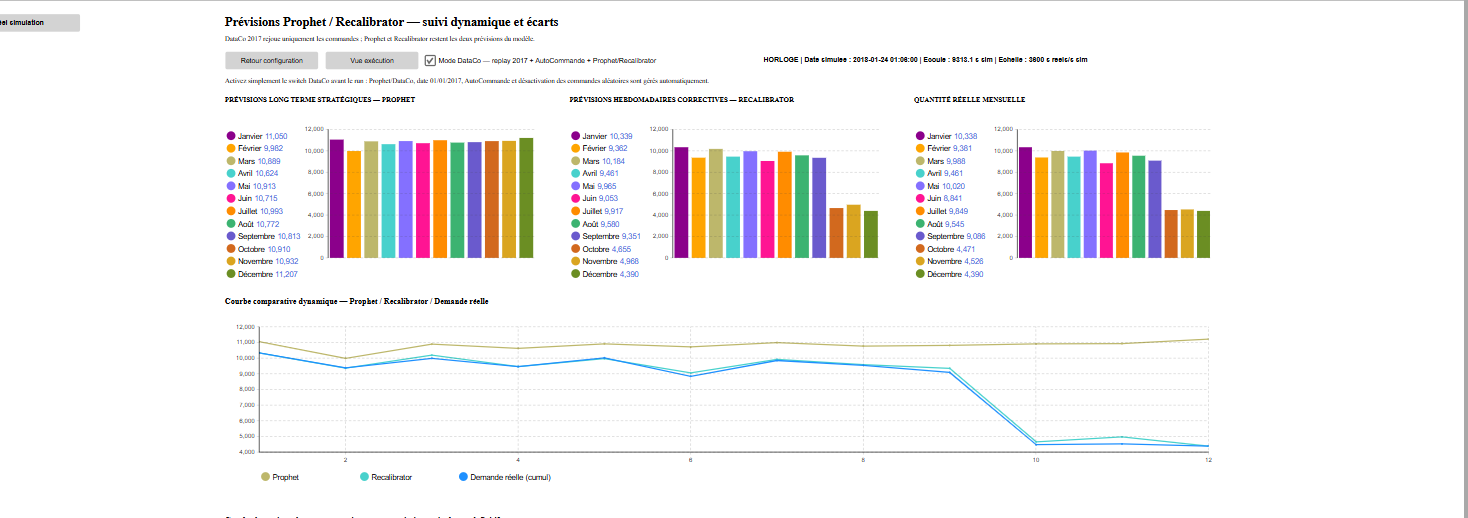
\includegraphics[width=\textwidth]{documentation/assets/dataco_final_run/screenshots/05_reference_dashboard_3600.png}
    \caption{Campagne DataCo de référence, \code{simToRealSeconds = 3600} : prévisions Prophet et Recalibrator mensuelles, demande réelle mensuelle et courbe comparative sur les douze mois (RUN 1).}
    \label{fig:interface-generale}
\end{figure}

Prophet constitue la référence stratégique initiale du modèle et reste stable tout au long de l'année, entre environ 9\,982 et 11\,207 unités mensuelles. La demande réelle observée pendant la campagne suit un comportement en deux phases : de janvier à septembre, elle oscille entre 8\,841 et 10\,338 unités par mois, proche de la prévision Prophet ; à partir d'octobre, elle se contracte fortement autour de 4\,400 unités mensuelles.

\begin{table}[htbp]
\centering
\caption{Prévisions Prophet et demande réelle mensuelle (RUN 1).}
\label{tab:prophet-reel}
\begin{tabular}{@{}lrr@{}}
\toprule
\textbf{Mois} & \textbf{Prophet} & \textbf{Demande réelle} \\
\midrule
Janvier & 11\,050 & 10\,338 \\
Février & 9\,982 & 9\,381 \\
Mars & 10\,889 & 9\,988 \\
Avril & 10\,624 & 9\,461 \\
Mai & 10\,913 & 10\,020 \\
Juin & 10\,715 & 8\,841 \\
Juillet & 10\,993 & 9\,849 \\
Août & 10\,772 & 9\,545 \\
Septembre & 10\,813 & 9\,086 \\
Octobre & 10\,910 & 4\,471 \\
Novembre & 10\,932 & 4\,526 \\
Décembre & 11\,207 & 4\,390 \\
\bottomrule
\end{tabular}
\end{table}

Le dernier trimestre porte la rupture la plus marquée de la campagne : en octobre, la demande réelle s'établit à 4\,471 unités alors que Prophet maintient une anticipation de 10\,910 unités. Le même écart se prolonge en novembre et en décembre. Prophet demeure une référence stratégique utile sur l'ensemble de l'année, et cette rupture de fin d'année illustre précisément la situation pour laquelle la recalibration adaptative apporte sa contribution la plus nette : elle ne doit pas être lue comme une saisonnalité structurelle reproductible d'une année sur l'autre, mais comme le test le plus exigeant du mécanisme de recalibration sur cette campagne.

\subsection{Prévision recalibrée}

\begin{figure}[htbp]
    \centering
    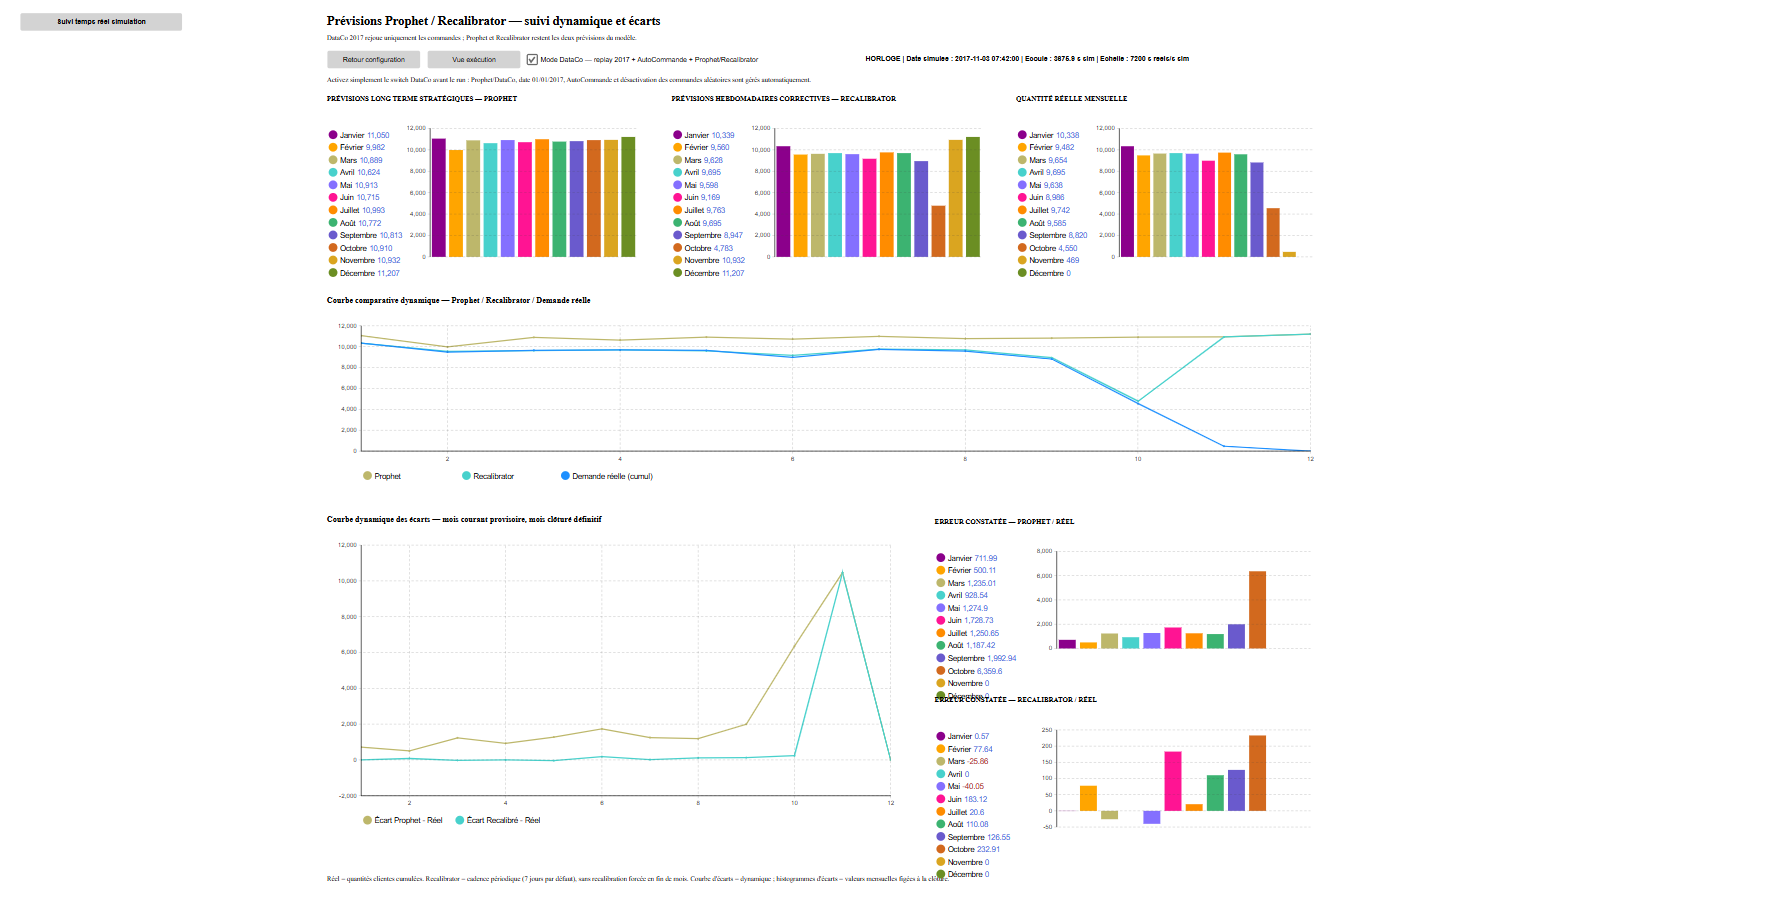
\includegraphics[width=\textwidth]{documentation/assets/dataco_final_run/screenshots/04_october_break.png}
    \caption{Contraction de la demande d'octobre-novembre et réaction du Recalibrator. Capture issue du run d'illustration accéléré (\code{simToRealSeconds = 7200,} RUN 2) : elle sert d'illustration de l'interface et de la dynamique du mécanisme, et non de source des valeurs numériques, qui restent celles du RUN 1 présentées dans cette section.}
    \label{fig:dashboard-rupture}
\end{figure}

Les valeurs recalibrées restent proches du réel sans s'y confondre systématiquement, avec des écarts mensuels alternativement positifs et négatifs : +0,57 en janvier, -18,53 en février, +195,93 en mars, 0 en avril, -55,38 en mai, +212 en juin, +68,11 en juillet, +35,43 en août, +265,28 en septembre, +183,71 en octobre, +441,74 en novembre et 0 en décembre. Les valeurs négatives de février et mai montrent que le mécanisme peut également corriger la prévision vers le bas lorsque la demande observée est inférieure à Prophet.

Jusqu'en septembre, Prophet reste généralement au-dessus du réel tandis que le Recalibrator suit plus étroitement les fluctuations mensuelles ; la différence devient particulièrement nette au dernier trimestre. En octobre :
\begin{align*}
F_{Prophet} &\approx 10\,910, \\
R_{\text{réel}} &= 4\,471, \\
F_{Recal} &\approx 4\,655.
\end{align*}
L'erreur Prophet atteint alors environ 6\,438,6 unités, contre environ 183,71 unités pour le Recalibrator. Le même phénomène se reproduit en novembre et en décembre : la recalibration corrige progressivement une prévision stratégique devenue obsolète dès que les observations signalent un changement de régime.

\subsection{Analyse quantitative des erreurs}

\begin{figure}[htbp]
    \centering
    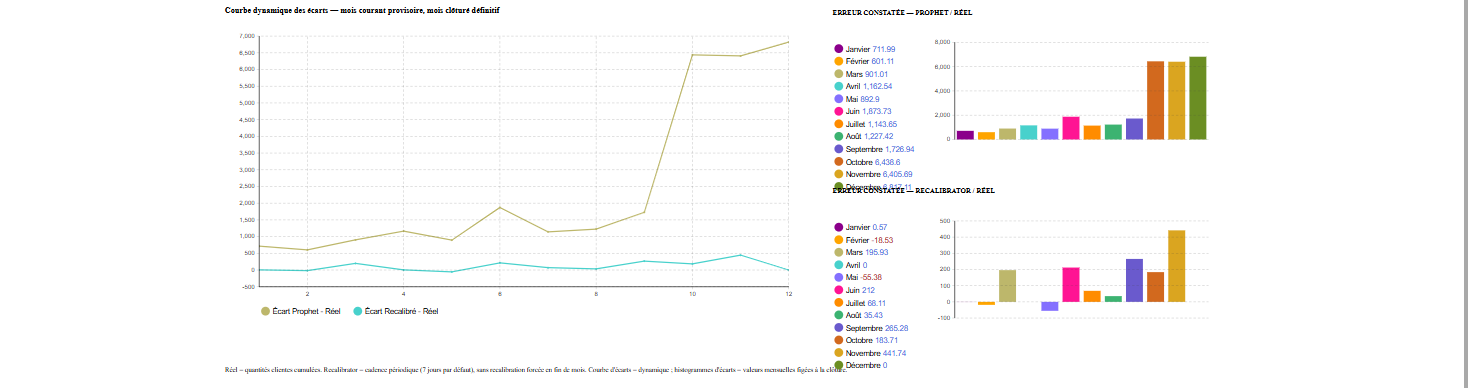
\includegraphics[width=\textwidth]{documentation/assets/dataco_final_run/screenshots/06_reference_errors_3600.png}
    \caption{Bilan Prophet / Recalibrator / demande réelle : courbe dynamique des écarts et histogrammes d'erreur mensuelle Prophet/Réel et Recalibrator/Réel, campagne de référence RUN 1 (\code{simToRealSeconds = 3600}).}
    \label{fig:dashboard-bilan}
\end{figure}

\begin{table}[htbp]
\centering
\caption{Erreurs mensuelles observées sur la campagne 2017 (RUN 1).}
\label{tab:erreurs-mensuelles}
\begin{tabular}{@{}lrr@{}}
\toprule
\textbf{Mois} & \textbf{Erreur Prophet / Réel} & \textbf{Erreur Recalibrator / Réel} \\
\midrule
Janvier & +711,99 & +0,57 \\
Février & +601,11 & -18,53 \\
Mars & +901,01 & +195,93 \\
Avril & +1\,162,54 & 0,00 \\
Mai & +892,90 & -55,38 \\
Juin & +1\,873,73 & +212,00 \\
Juillet & +1\,143,65 & +68,11 \\
Août & +1\,227,42 & +35,43 \\
Septembre & +1\,726,94 & +265,28 \\
Octobre & +6\,438,60 & +183,71 \\
Novembre & +6\,405,69 & +441,74 \\
Décembre & +6\,817,11 & 0,00 \\
\bottomrule
\end{tabular}
\end{table}

Prophet présente une erreur positive sur les douze mois de la campagne, ce qui traduit un biais de surestimation sur ce run. Le Recalibrator réduit fortement cette erreur et corrige également vers le bas en février et en mai. Les valeurs nulles d'avril et décembre résultent de la coïncidence entre une échéance de recalibration et la clôture du mois.

\begin{table}[htbp]
\centering
\caption{Synthèse des performances de prévision sur la campagne DataCo 2017 (RUN 1).}
\label{tab:metriques-prevision}
\begin{tabular}{@{}lrrl@{}}
\toprule
\textbf{Indicateur} & \textbf{Prophet} & \textbf{Recalibrator} & \textbf{Réduction} \\
\midrule
Erreur absolue totale & 29\,902,69 & 1\,476,68 & -95,1\,\% \\
MAE mensuelle & 2\,491,89 & 123,06 & -95,1\,\% \\
MAPE & 45,75\,\% & 1,91\,\% & -43,8 points \\
RMSE & 3\,441,15 & 180,71 & -94,7\,\% \\
Biais moyen signé & +2\,491,89 & +110,74 & -95,6\,\% \\
\bottomrule
\end{tabular}
\end{table}

Pour chaque indicateur, la lecture est directe : la MAE mensuelle passe de 2\,491,89 à 123,06 unités, soit une réduction de 95,1\,\% de l'erreur moyenne absolue ; le MAPE passe de 45,75\,\% à 1,91\,\%, ce qui signifie que la prévision s'écarte désormais en moyenne de 1,9\,\% de la demande réelle contre 45,8\,\% initialement ; le RMSE passe de 3\,441,15 à 180,71, confirmant que les écarts ponctuels de grande amplitude du dernier trimestre sont ramenés à un niveau proche de ceux des autres mois. La réduction relative de l'erreur absolue totale s'établit à :
\[
\mathcal{R} = 1 - \frac{1\,476{,}68}{29\,902{,}69} \approx 95{,}06\,\%, \qquad
\frac{29\,902{,}69}{1\,476{,}68} \approx 20{,}25
\]
soit environ 20,25 fois moins d'erreur absolue cumulée pour le Recalibrator que pour Prophet sur cette campagne.

\subsection{Interprétation opérationnelle}

Cette amélioration se traduit directement en termes opérationnels. Dans un contexte de production sur stock, une surestimation de plusieurs milliers d'unités conduit à augmenter inutilement le niveau de stock, à déclencher des réapprovisionnements excessifs, à mobiliser la capacité de production et à accroître le risque d'invendus ; une sous-estimation trop marquée augmente à l'inverse le risque de rupture et de retard de service. Le mois d'octobre illustre cet enjeu : Prophet projette environ 10\,910 unités pour une demande réelle de 4\,471 unités, une surestimation supérieure à 6\,400 unités, que le Recalibrator ramène à un écart d'environ 183,71 unités. La contribution du Recalibrator ne réside donc pas dans une prévision parfaitement exacte, mais dans sa capacité à corriger rapidement une décision stratégique lorsque la demande observée s'écarte durablement du régime anticipé.

\subsection{Résultats opérationnels complémentaires}

Le snapshot synchronisé avec l'export ontologique du RUN 1 indique un Performance Index global de \(8{,}871/10\) et recense 79 commandes clientes closes au moment du relevé, dont 20 closes en retard, sur les 365 commandes générées par la campagne de demande ; 286 commandes restent EN\_ATTENTE. La date simulée de cet export de clôture est le 14 mars 2018. Cet écart est cohérent avec la poursuite du traitement physique au-delà de la fin de la campagne de génération de la demande : les résultats Prophet et Recalibrator sont d'ores et déjà évaluables sur les douze mois, car ils portent sur la demande client reçue, tandis que les indicateurs de service, de délai et de livraison se consolident au rythme de l'extinction complète des flux résiduels.

\textbf{Condition terminale.} La fin de la campagne de demande -- 365 jours, 365 commandes générées -- ne correspond pas à l'état terminal opérationnel du système : ce dernier suppose que toutes les commandes clientes sont closes, que tous les ordres internes de réapprovisionnement sont terminés, et qu'aucun encours pertinent ne subsiste. Un Performance Index ou des KPI relevés avant cet état, comme le snapshot à 79 commandes closes sur 365 ci-dessus, constituent donc un \emph{snapshot intermédiaire} et non un bilan terminal. Cette distinction est essentielle pour l'expérimentation E5 (section~\ref{sec:optimisation}), dont les résultats terminaux doivent être mesurés après extinction complète des flux résiduels.

\textbf{Backlog et réapprovisionnement.} Trois constats distincts doivent être distingués, comme détaillé table~\ref{tab:dataco-statuts-commandes}. Les retards clôturés (20 commandes closes en retard) sont exclusivement portés par DATACO\_SPORTS. Le réapprovisionnement autonome REAPPRO\_4 (19\,770 unités) est également EN\_COURS sur DATACO\_SPORTS au moment du relevé. Le backlog client encore EN\_ATTENTE, en revanche, est réparti sur les trois familles (79 commandes sur DATACO\_SPORTS, 104 sur DATACO\_CLOTHING, 103 sur DATACO\_ELECTRONICS) : REAPPRO\_4 n'est donc pas présenté comme la cause démontrée de l'ensemble du backlog, seulement comme l'ordre en cours identifié sur DATACO\_SPORTS. Dans cette configuration et au snapshot observé, le flux physique n'est pas encore éteint sur aucune des trois familles : la demande générée excède momentanément la capacité de reconstitution et de traitement du scénario courant, ce qui prolonge l'extinction des flux au-delà de la fin de la campagne calendaire. Le run d'illustration (RUN 2) présente un constat de même nature, avec un ordre de réapprovisionnement EN\_COURS de 16\,013 unités sur DATACO\_SPORTS. E5 permettra d'étudier les politiques de planification et de stock qui influent sur cette situation, famille par famille.

La campagne DataCo 2017 valide conjointement la génération automatique de la demande, le fonctionnement multi-produit, la séparation des stocks par référence, le déclenchement autonome des réapprovisionnements et la recalibration adaptative des prévisions. Prophet apporte une base stratégique stable ; le Recalibrator transfère progressivement la confiance vers les observations au fur et à mesure du déroulement du mois, ce qui maintient la cohérence entre planification et exécution lorsque le comportement de la demande diverge de la trajectoire anticipée.

\section{Perspectives d'amélioration}

Plusieurs directions permettent de prolonger la validation du module :
\begin{itemize}[leftmargin=1.5em]
  \item une analyse de sensibilité du facteur de confiance sur la famille \(\gamma \in \{0{,}3,\ 0{,}5,\ 0{,}7,\ 1{,}0\}\), en comparant pour chaque réglage la MAE, le RMSE, le MAPE et le biais moyen signé ;
  \item l'ajout de signaux exogènes -- promotions, météo, tendances externes -- en complément des commandes déjà observées ;
  \item une granularité plus fine de la prévision et de la recalibration, au niveau du produit plutôt qu'au niveau agrégé mensuel ;
  \item l'extension des politiques d'optimisation présentées section~\ref{sec:optimisation} à la planification multi-produit fondée sur la prévision ;
  \item une validation du module sur d'autres jeux de données et d'autres cas industriels que la campagne DataCo 2017.
\end{itemize}

\section{La phase d'optimisation}
\label{sec:optimisation}

La phase d'optimisation exploite les capacités de simulation et de mesure de SCONTO-SVU pour rechercher les configurations de décision les plus performantes dans un espace défini. Elle prolonge la chaîne de pilotage déjà en place -- simulation, diagnostic, comparaison, replanification -- par une recherche systématique de configuration, structurée en six éléments : des variables de décision, des fonctions objectives, des contraintes, une politique de référence, une méthode de recherche et une validation comparative et statistique.

\subsection{E4 -- Optimisation de la réponse au choc de demande chez ZENER}

\textbf{Baseline.} Le scénario perturbé E2 sert de politique de référence.

\textbf{Variables de décision.}
\begin{itemize}[leftmargin=1.5em]
  \item \(x_1\) : capacité du poste critique identifié lors du diagnostic E1/E2 ;
  \item \(x_2\) : fractionnement du lot (taille des sous-lots de production) ;
  \item \(x_3\) : règle de priorité appliquée au poste critique ;
  \item \(x_4\) : politique ou niveau de stock.
\end{itemize}

\textbf{Objectifs.} Minimiser le nombre de retards, minimiser le WIP moyen, minimiser le lead time / Order Fulfillment Cycle Time, minimiser le coût, maximiser le Performance Index.

\textbf{Contraintes.} Stock non négatif, capacité installée non dépassée, satisfaction de la demande dans les limites déjà définies par le modèle, budget si un budget est activé, niveau de service minimal si défini, et une règle de terminaison commune entre toutes les configurations comparées.

\textbf{Méthode de recherche.} Exploration factorielle des combinaisons \((x_1,x_2,x_3,x_4)\), construction d'un front de Pareto sur les cinq objectifs à partir des solutions admissibles, puis sélection d'une solution parmi les solutions Pareto-efficaces par AHP multi-experts : l'AHP sélectionne un compromis managérial parmi des solutions déjà Pareto-efficaces, en aval de la recherche d'optimisation proprement dite.

\subsection{E5 -- Optimisation de la planification multi-produit fondée sur la prévision}

\textbf{Avertissement.} L'expérimentation E5 n'a pas encore été exécutée. Elle est présentée ici comme un protocole expérimental à exécuter, formalisé selon les mêmes exigences que E4 : variables de décision, fonction objective, contraintes, politique de référence et méthode de recherche.

Cette extension compare quatre politiques de pilotage :

\begin{center}
\begin{tabularx}{0.92\textwidth}{lX}
\toprule
Politique & Description \\
\midrule
P0 & Réactive, sans prévision (référence) \\
P1 & Pilotée par Prophet seul \\
P2 & Pilotée par Prophet et Recalibrator \\
P3 & Pilotée par Prophet, Recalibrator et paramètres de planification et de stock optimisés selon le protocole E5 \\
\bottomrule
\end{tabularx}
\end{center}

E4 fournit une démarche générale de simulation-optimisation ; E5 possède son propre espace de décision, propre à la planification multi-produit fondée sur la prévision.

\textbf{Variables de décision.} Pour chaque famille simulée \(p\) (section~\ref{sec:dataco-dataset}), le vecteur de décision est
\[
x_p = (SS_p,\; s_p,\; Q_p,\; f_p)
\]
où \(SS_p\) est le stock de sécurité de la famille, \(s_p\) le point de commande, \(Q_p\) la quantité de réapprovisionnement et \(f_p\) la fréquence de révision du plan. L'espace de décision complet est l'ensemble des vecteurs \((x_p)_{p \in P}\) pour les familles simulées.

\textbf{Fonction objective.} L'optimisation recherche la configuration minimisant le coût total cumulé sur l'horizon de simulation :
\[
\min\; C_{\text{total}} = \sum_{p,t} \Big[ h_p\, I_{p,t} + b_p\, B_{p,t} + K_p\, y_{p,t} + c_p\, Q_{p,t} \Big]
\]
où \(I_{p,t}\) est le niveau de stock de la famille \(p\) en fin de période \(t\), \(B_{p,t}\) la rupture ou le retard cumulé, \(y_{p,t}\) une variable indicatrice de déclenchement d'un ordre de réapprovisionnement, et \(h_p\), \(b_p\), \(K_p\), \(c_p\) respectivement le coût de possession, le coût de rupture, le coût fixe de commande et le coût unitaire de la famille \(p\).

\textbf{Contraintes.} La recherche est contrainte par :
\begin{itemize}[leftmargin=1.5em]
  \item un niveau de service minimal par famille, \(\text{NiveauDeService}_p \geq SL_p^{\min}\) ;
  \item une capacité de réapprovisionnement bornée par période, \(Q_{p,t} \leq \text{Capacite}_{p,t}\) ;
  \item une équation de bilan de stock, \(I_{p,t} = I_{p,t-1} + Q_{p,t} - D_{p,t}\), où \(D_{p,t}\) est la demande de la famille \(p\) sur la période \(t\), issue de la chaîne de prévision et de recalibration décrite aux sections~\ref{sec:prophet} et~\ref{sec:recalibrator}.
\end{itemize}

\textbf{Chaîne prévision-plan-exécution-performance.} Chaque politique P1 à P3 s'inscrit dans une chaîne où la prévision (Prophet, éventuellement recalibrée) alimente un plan de réapprovisionnement par famille, ce plan est exécuté par la simulation multi-produit selon les mécanismes DataCo et AutoCommande déjà décrits (section~\ref{sec:autocommande}), et la performance résultante n'est mesurable qu'à la condition terminale du run, telle que définie plus haut. Comparer des politiques sur un état intermédiaire biaiserait l'évaluation du coût total \(C_{\text{total}}\), notamment sa composante rupture \(B_{p,t}\), qui dépend de l'historique complet du run.

\subsection{Plan de validation}

\textbf{Prérequis technique.} La mise en \oe uvre des nombres aléatoires communs suppose d'exposer et de contrôler explicitement la graine de génération aléatoire de l'expérience AnyLogic avant la campagne d'optimisation. Ce contrôle n'est pas acquis dans l'état actuel : le manifeste runtime des campagnes RUN 1 et RUN 2 indique \code{graineAleatoire = NON\_ACCESSIBLE\_DANS\_MAIN}, ce qui signifie que la graine effectivement utilisée par ces deux runs n'a pas pu être lue ni contrôlée depuis \code{Main}. Le protocole de graines communes décrit ci-dessous doit donc être considéré comme une exigence à mettre en place, et non comme un mécanisme déjà opérationnel sur les runs déjà exécutés.

Pour toute configuration retenue en E4 ou E5, la validation prévoit plusieurs réplications par configuration, avec des graines aléatoires communes entre configurations comparées : pour une réplication \(k\), la graine appliquée à la politique de référence \(P_0\) et celle appliquée à une politique alternative \(P_i\) satisfont \(\text{Seed}_{k,P_0} = \text{Seed}_{k,P_i}\), de sorte que les différences observées entre politiques ne soient pas imputables à un tirage aléatoire différent. Le nombre de réplications retenu suit une règle d'arrêt fondée sur la précision de l'estimation : les réplications se poursuivent jusqu'à ce que la demi-largeur de l'intervalle de confiance à 95\,\% du critère principal (par exemple le Performance Index ou \(C_{\text{total}}\)) descende sous un seuil fixé a priori, par exemple 5\,\% de la valeur moyenne estimée. Une validation croisée est ensuite conduite sur de nouvelles graines, indépendantes de celles utilisées pour la sélection de la configuration, afin d'écarter un ajustement optimiste aux réplications d'exploration.

Pour chaque comparaison, sont rapportés conjointement la moyenne et l'écart-type du critère sur les réplications, l'intervalle de confiance à 95\,\%, la différence absolue et relative par rapport à la politique de référence, un test statistique apparié adapté au plan d'expérience à graines communes, une taille d'effet complémentaire à la significativité statistique, et une vérification de robustesse sur plusieurs intensités de perturbation de la demande. Une configuration retenue à l'issue de ce protocole est qualifiée de meilleure configuration identifiée dans l'espace de décisions exploré, et non d'optimum global.

\section{Interprétation expérimentale}

Le module conduit une expérience complète, de bout en bout :
\[
\boxed{\text{Prévision Prophet} \longrightarrow \text{Demande DataCo exécutée} \longrightarrow \text{Réel observé} \longrightarrow \text{Recalibration}}
\]

Cette chaîne permet d'étudier la capacité d'une prévision initiale à rester pertinente lorsqu'une demande simulée se matérialise, puis de mesurer dans quelle mesure un mécanisme adaptatif améliore cette prévision. Le même socle sert à comparer plusieurs stratégies de pilotage -- demande réelle observée, Prophet seul, ou Prophet recalibré -- avec évaluation des impacts sur le stock, les ruptures, le taux de service, les délais et les KPI SCOR. Le module reste analytique et non intrusif sur les politiques de stock, ce qui facilite sa validation sans remettre en cause le comportement physique déjà approuvé du modèle.

\section{Résumé}

Le module ajouté à SCONTO-SVU repose sur trois rôles complémentaires : \textbf{Prophet} fournit la prévision mensuelle de référence ; \textbf{DataCo} exécute la demande sous forme de commandes clientes journalières qui traversent le pipeline normal ; \textbf{Recalibrator} ajuste progressivement la prévision à partir du réel observé. Sur la campagne DataCo 2017 (RUN 1, \code{simToRealSeconds = 3600}), l'erreur absolue totale est réduite de 95,1\,\%, la MAE mensuelle passe de 2\,492 à 123 unités et le MAPE passe de 45,8\,\% à 1,9\,\%.

La vue dédiée rend ces mécanismes observables en temps réel grâce à trois courbes principales, deux courbes d'écarts dynamiques et une horloge simulée synchronisée avec l'échelle temporelle du modèle, ce qui fournit une base cohérente pour l'analyse prévisionnelle, l'étude des écarts et les expérimentations de pilotage de la supply chain.

\begin{thebibliography}{9}

\bibitem{dataco2019}
Constante, F., Silva, F., \& Pereira, A. (2019). \emph{DataCo Smart Supply Chain for Big Data Analysis}. Mendeley Data ; distribué également via Kaggle (2019).

\bibitem{taylor2018forecasting}
Taylor, S. J., \& Letham, B. (2018). Forecasting at Scale. \emph{The American Statistician}, 72(1), 37--45. DOI: 10.1080/00031305.2017.1380080.

\bibitem{prophetdocs}
Prophet -- documentation officielle du logiciel, \url{https://facebook.github.io/prophet/}.

\bibitem{batesgranger1969}
Bates, J. M., \& Granger, C. W. J. (1969). The Combination of Forecasts. \emph{Operational Research Quarterly}, 20(4), 451--468.

\bibitem{timmermann2006}
Timmermann, A. (2006). Forecast Combinations. In G. Elliott, C. W. J. Granger, \& A. Timmermann (Eds.), \emph{Handbook of Economic Forecasting}, Vol. 1, 135--196. Elsevier.

\bibitem{brown1956}
Brown, R. G. (1956). \emph{Exponential Smoothing for Predicting Demand}. Arthur D. Little Inc.

\bibitem{holtwinters1960}
Holt, C. C. (1957/2004 réédition). Forecasting seasonals and trends by exponentially weighted moving averages. \emph{International Journal of Forecasting}, 20(1), 5--10 ; Winters, P. R. (1960). Forecasting Sales by Exponentially Weighted Moving Averages. \emph{Management Science}, 6(3), 324--342.

\bibitem{hadleywhitin1963}
Hadley, G., \& Whitin, T. M. (1963). \emph{Analysis of Inventory Systems}. Prentice-Hall, Englewood Cliffs, N.J.

\end{thebibliography}

\end{document}
